\documentclass[a4paper]{scrreprt}

%% Language and font encodings and page settings
\usepackage[english]{babel}
\usepackage[utf8x]{inputenc}
\usepackage[T1]{fontenc}
\usepackage[a4paper,top=3cm,bottom=2cm,left=3cm,right=3cm,marginparwidth=2cm]{geometry}

%% Packages
\usepackage{amsmath}
\usepackage{graphicx}
\usepackage[colorinlistoftodos]{todonotes}
\usepackage[colorlinks=true, allcolors=blue]{hyperref}

\title{Brexit Vs Good Friday}
\subtitle{"Defend the Good Friday Agreement"}
\author{Cian Gannon}
\titlehead{\centering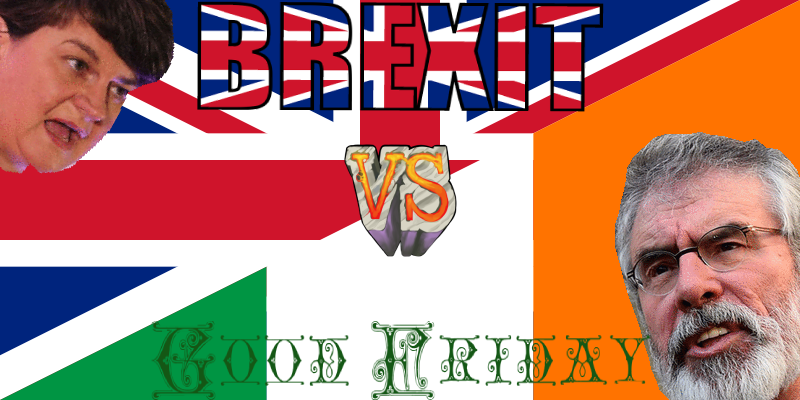
\includegraphics[width=10cm]{header}}

\pagestyle{headings}

\begin{document}

    \maketitle

    \begin{abstract}
        
        Brexit Vs Good Friday is a satirical representation of the current Brexit debacle and Ireland's core involvement in it due to the Good Friday Agreement. 
        Brexit Vs Good Friday is a top-down shooter that will expand the genre and also involve the most loved elements of other shooters.
        
    \end{abstract}

    \tableofcontents

    \chapter{Overview}

    \section{Main Concept}
    Brexit Vs Good Friday is a satirical representation of Brexit and the hysteria surrounding it. It's a top down shooter where the user plays Gerry Adams a politician who returns from retirement in order to save what many hold dear.
    
    \section{Core Selling Points}

        \subsection{Survival}
            \begin{description}
                \item[$\bullet$] Player must dodge incoming fire.
                \item[$\bullet$] The aim of the game is to protect Good Friday in a countdown until the UK leaves the EU and the single market. If the player fails in their attempt by getting hit then Good Friday will be removed and the player fails. If the player survives the countdown then the Good Friday is upheld.
            \end{description}
        
        \subsection{Humor}
            \begin{description}
                \item[$\bullet$] The game is made to be humorous. It's take on Brexit that is a core issue currently in the EU is used to make all players on both sides laugh.
                \item[$\bullet$] The game is created to be topical, games that are topical tend to be a hit with players.
            \end{description}

        \subsection{Top Down Shooter}
            \begin{description}
                \item[$\bullet$] Top down shooter which needs basic input so the game will be comfortable to play on mobile or desktop.
                \item[$\bullet$] Top down games have been around for generations of consoles and have evolved over time. Brexit Vs Good Friday aims to take the general style and improve upon it.
            \end{description}
\end{document}